\upaper{111}{The Adjuster and the Soul}
\author{Solitary Messenger}
\vs p111 0:1 The presence of the divine Adjuster in the human mind makes it forever impossible for either science or philosophy to attain a satisfactory comprehension of the evolving soul of the human personality. The morontia soul is the child of the universe and may be really known only through cosmic insight and spiritual discovery.
\vs p111 0:2 \pc The concept of a soul and of an indwelling spirit is not new to Urantia; it has frequently appeared in the various systems of planetary beliefs. Many of the Oriental as well as some of the Occidental faiths have perceived that man is divine in heritage as well as human in inheritance. The feeling of the inner presence in addition to the external omnipresence of Deity has long formed a part of many Urantian religions. Men have long believed that there is something growing within the human nature, something vital that is destined to endure beyond the short span of temporal life.
\vs p111 0:3 Before man realized that his evolving soul was fathered by a divine spirit, it was thought to reside in different physical organs --- the eye, liver, kidney, heart, and later, the brain. The savage associated the soul with blood, breath, shadows and with reflections of the self in water.
\vs p111 0:4 In the conception of the \bibemph{atman} the Hindu teachers really approximated an appreciation of the nature and presence of the Adjuster, but they failed to distinguish the copresence of the evolving and potentially immortal soul. The Chinese, however, recognized two aspects of a human being, the \bibemph{yang} and the \bibemph{yin,} the soul and the spirit. The Egyptians and many African tribes also believed in two factors, the \bibemph{ka} and the \bibemph{ba;} the soul was not usually believed to be pre\hyp{}existent, only the spirit.
\vs p111 0:5 The inhabitants of the Nile valley believed that each favoured individual had bestowed upon him at birth, or soon thereafter, a protecting spirit which they called the ka. They taught that this guardian spirit remained with the mortal subject throughout life and passed before him into the future estate. On the walls of a temple at Luxor, where is depicted the birth of Amenhotep III, the little prince is pictured on the arm of the Nile god, and near him is another child, in appearance identical with the prince, which is a symbol of that entity which the Egyptians called the ka. This sculpture was completed in the XV century before Christ.\tunemarkup{pictures}{\begin{figure}[H]\centering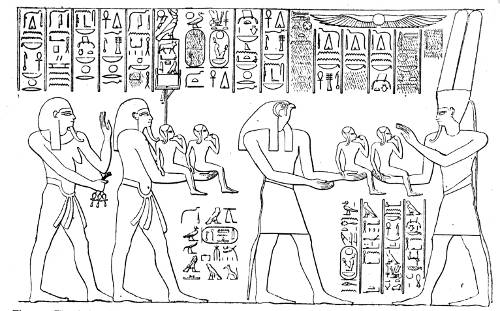
\includegraphics[width=\columnwidth]{images/AmenhotepIII-and-his-Ka.jpg}\caption{The infant king, Amenophis III and his Ka, presented to Amen Rā, the god of Thebes, by two Nile gods, and by Horus. \bibemph{From the temple of Amenophis III, at Luxor.}}\end{figure}}
\vs p111 0:6 The ka was thought to be a superior spirit genius which desired to guide the associated mortal soul into the better paths of temporal living but more especially to influence the fortunes of the human subject in the hereafter. When an Egyptian of this period died, it was expected that his ka would be waiting for him on the other side of the Great River. At first, only kings were supposed to have kas, but presently all righteous men were believed to possess them. One Egyptian ruler, speaking of the ka within his heart, said: “I did not disregard its speech; I feared to transgress its guidance. I prospered thereby greatly; I was thus successful by reason of that which it caused me to do; I was distinguished by its guidance.” Many believed that the ka was “an oracle from God in everybody.” Many believed that they were to “spend eternity in gladness of heart in the favour of the God that is in you.”
\vs p111 0:7 Every race of evolving Urantia mortals has a word equivalent to the concept of soul. Many primitive peoples believed the soul looked out upon the world through human eyes; therefore did they so cravenly fear the malevolence of the evil eye. They have long believed that “the spirit of man is the lamp of the Lord.” The Rig\hyp{}Veda says: “My mind speaks to my heart.”
\usection{1.\bibnobreakspace The Mind Arena of Choice}
\vs p111 1:1 Though the work of Adjusters is spiritual in nature, they must, perforce, do all their work upon an intellectual foundation. Mind is the human soil from which the spirit Monitor must evolve the morontia soul with the co\hyp{}operation of the indwelt personality.
\vs p111 1:2 There is a cosmic unity in the several mind levels of the universe of universes. Intellectual selves have their origin in the cosmic mind much as nebulae take origin in the cosmic energies of universe space. On the human (hence personal) level of intellectual selves the potential of spirit evolution becomes dominant, with the assent of the mortal mind, because of the spiritual endowments of the human personality together with the creative presence of an entity\hyp{}point of absolute value in such human selves. But such a spirit dominance of the material mind is conditioned upon two experiences: This mind must have evolved up through the ministry of the seven adjutant mind\hyp{}spirits, and the material (personal) self must choose to co\hyp{}operate with the indwelling Adjuster in creating and fostering the morontia self, the evolutionary and potentially immortal soul.
\vs p111 1:3 \pc Material mind is the arena in which human personalities live, are self\hyp{}conscious, make decisions, choose God or forsake him, eternalize or destroy themselves.
\vs p111 1:4 \pc Material evolution has provided you a life machine, your body; the Father himself has endowed you with the purest spirit reality known in the universe, your Thought Adjuster. But into your hands, subject to your own decisions, has been given mind, and it is by mind that you live or die. It is within this mind and with this mind that you make those moral decisions which enable you to achieve Adjusterlikeness, and that is Godlikeness.
\vs p111 1:5 Mortal mind is a temporary intellect system loaned to human beings for use during a material lifetime, and as they use this mind, they are either accepting or rejecting the potential of eternal existence. Mind is about all you have of universe reality that is subject to your will, and the soul --- the morontia self --- will faithfully portray the harvest of the temporal decisions which the mortal self is making. Human consciousness rests gently upon the electrochemical mechanism below and delicately touches the spirit\hyp{}morontia energy system above. Of neither of these two systems is the human being ever completely conscious in his mortal life; therefore must he work in mind, of which he is conscious. And it is not so much what mind comprehends as what mind desires to comprehend that ensures survival; it is not so much what mind is like as what mind is striving to be like that constitutes spirit identification. It is not so much that man is conscious of God as that man yearns for God that results in universe ascension. What you are today is not so important as what you are becoming day by day and in eternity.
\vs p111 1:6 Mind is the cosmic instrument on which the human will can play the discords of destruction, or upon which this same human will can bring forth the exquisite melodies of God identification and consequent eternal survival. The Adjuster bestowed upon man is, in the last analysis, impervious to evil and incapable of sin, but mortal mind can actually be twisted, distorted, and rendered evil and ugly by the sinful machinations of a perverse and self\hyp{}seeking human will. Likewise can this mind be made noble, beautiful, true, and good --- actually great --- in accordance with the spirit\hyp{}illuminated will of a God\hyp{}knowing human being.
\vs p111 1:7 \pc Evolutionary mind is only fully stable and dependable when manifesting itself upon the two extremes of cosmic intellectuality --- the wholly mechanized and the entirely spiritualized. Between the intellectual extremes of pure mechanical control and true spirit nature there intervenes that enormous group of evolving and ascending minds whose stability and tranquillity are dependent upon personality choice and spirit identification.
\vs p111 1:8 But man does not passively, slavishly, surrender his will to the Adjuster. Rather does he actively, positively, and co\hyp{}operatively choose to follow the Adjuster’s leading when and as such leading consciously differs from the desires and impulses of the natural mortal mind. The Adjusters manipulate but never dominate man’s mind against his will; to the Adjusters the human will is supreme. And they so regard and respect it while they strive to achieve the spiritual goals of thought adjustment and character transformation in the almost limitless arena of the evolving human intellect.
\vs p111 1:9 \pc Mind is your ship, the Adjuster is your pilot, the human will is captain. The master of the mortal vessel should have the wisdom to trust the divine pilot to guide the ascending soul into the morontia harbours of eternal survival. Only by selfishness, slothfulness, and sinfulness can the will of man reject the guidance of such a loving pilot and eventually wreck the mortal career upon the evil shoals of rejected mercy and upon the rocks of embraced sin. With your consent, this faithful pilot will safely carry you across the barriers of time and the handicaps of space to the very source of the divine mind and on beyond, even to the Paradise Father of Adjusters.
\usection{2.\bibnobreakspace Nature of the Soul}
\vs p111 2:1 Throughout the mind functions of cosmic intelligence, the totality of mind is dominant over the parts of intellectual function. Mind, in its essence, is functional unity; therefore does mind never fail to manifest this constitutive unity, even when hampered and hindered by the unwise actions and choices of a misguided self. And this unity of mind invariably seeks for spirit co\hyp{}ordination on all levels of its association with selves of will dignity and ascension prerogatives.
\vs p111 2:2 The material mind of mortal man is the cosmic loom that carries the morontia fabrics on which the indwelling Thought Adjuster threads the spirit patterns of a universe character of enduring values and divine meanings --- a surviving soul of ultimate destiny and unending career, a potential finaliter.
\vs p111 2:3 The human personality is identified with mind and spirit held together in functional relationship by life in a material body. This functioning relationship of such mind and spirit does not result in some combination of the qualities or attributes of mind and spirit but rather in an entirely new, original, and unique universe value of potentially eternal endurance, the \bibemph{soul.}
\vs p111 2:4 \pc There are three and not two factors in the evolutionary creation of such an immortal soul. These three antecedents of the morontia human soul are:
\vs p111 2:5 \ublistelem{1.}\bibnobreakspace \bibemph{The human mind} and all cosmic influences antecedent thereto and impinging thereon.
\vs p111 2:6 \ublistelem{2.}\bibnobreakspace \bibemph{The divine spirit} indwelling this human mind and all potentials inherent in such a fragment of absolute spirituality together with all associated spiritual influences and factors in human life.
\vs p111 2:7 \ublistelem{3.}\bibnobreakspace \bibemph{The relationship between material mind and divine spirit,} which connotes a value and carries a meaning not found in either of the contributing factors to such an association. The reality of this unique relationship is neither material nor spiritual but morontial. It is the soul.
\vs p111 2:8 \pc The midway creatures have long denominated this evolving soul of man the mid\hyp{}mind in contradistinction to the lower or material mind and the higher or cosmic mind. This mid\hyp{}mind is really a morontia phenomenon since it exists in the realm between the material and the spiritual. The potential of such a morontia evolution is inherent in the two universal urges of mind: the impulse of the finite mind of the creature to know God and attain the divinity of the Creator, and the impulse of the infinite mind of the Creator to know man and attain the \bibemph{experience} of the creature.
\vs p111 2:9 This supernal transaction of evolving the immortal soul is made possible because the mortal mind is first personal and second is in contact with superanimal realities; it possesses a supermaterial endowment of cosmic ministry which ensures the evolution of a moral nature capable of making moral decisions, thereby effecting a bona fide creative contact with the associated spiritual ministries and with the indwelling Thought Adjuster.
\vs p111 2:10 The inevitable result of such a contactual spiritualization of the human mind is the gradual birth of a soul, the joint offspring of an adjutant mind dominated by a human will that craves to know God, working in liaison with the spiritual forces of the universe which are under the overcontrol of an actual fragment of the very God of all creation --- the Mystery Monitor. And thus does the material and mortal reality of the self transcend the temporal limitations of the physical\hyp{}life machine and attain a new expression and a new identification in the evolving vehicle for selfhood continuity, the morontia and immortal soul.
\usection{3.\bibnobreakspace The Evolving Soul}
\vs p111 3:1 The mistakes of mortal mind and the errors of human conduct may markedly delay the evolution of the soul, although they cannot inhibit such a morontia phenomenon when once it has been initiated by the indwelling Adjuster with the consent of the creature will. But at any time prior to mortal death this same material and human will is empowered to rescind such a choice and to reject survival. Even after survival the ascending mortal still retains this prerogative of choosing to reject eternal life; at any time before fusion with the Adjuster the evolving and ascending creature can choose to forsake the will of the Paradise Father. Fusion with the Adjuster signalizes the fact that the ascending mortal has eternally and unreservedly chosen to do the Father’s will.
\vs p111 3:2 During the life in the flesh the evolving soul is enabled to reinforce the supermaterial decisions of the mortal mind. The soul, being supermaterial, does not of itself function on the material level of human experience. Neither can this subspiritual soul, without the collaboration of some spirit of Deity, such as the Adjuster, function above the morontia level. Neither does the soul make final decisions until death or translation divorces it from material association with the mortal mind except when and as this material mind delegates such authority freely and willingly to such a morontia soul of associated function. During life the mortal will, the personality power of decision\hyp{}choice, is resident in the material mind circuits; as terrestrial mortal growth proceeds, this self, with its priceless powers of choice, becomes increasingly identified with the emerging morontia\hyp{}soul entity; after death and following the mansion world resurrection, the human personality is completely identified with the morontia self. The soul is thus the embryo of the future morontia vehicle of personality identity.
\vs p111 3:3 This immortal soul is at first wholly morontia in nature, but it possesses such a capacity for development that it invariably ascends to the true spirit levels of fusion value with the spirits of Deity, usually with the same spirit of the Universal Father that initiated such a creative phenomenon in the creature mind.
\vs p111 3:4 Both the human mind and the divine Adjuster are conscious of the presence and differential nature of the evolving soul --- the Adjuster fully, the mind partially. The soul becomes increasingly conscious of both the mind and the Adjuster as associated identities, proportional to its own evolutionary growth. The soul partakes of the qualities of both the human mind and the divine spirit but persistently evolves toward augmentation of spirit control and divine dominance through the fostering of a mind function whose meanings seek to co\hyp{}ordinate with true spirit value.
\vs p111 3:5 The mortal career, the soul’s evolution, is not so much a probation as an education. Faith in the survival of supreme values is the core of religion; genuine religious experience consists in the union of supreme values and cosmic meanings as a realization of universal reality.
\vs p111 3:6 Mind knows quantity, reality, meanings. But quality --- values --- is \bibemph{felt.} That which feels is the mutual creation of mind, which knows, and the associated spirit, which reality\hyp{}izes.
\vs p111 3:7 In so far as man’s evolving morontia soul becomes permeated by truth, beauty, and goodness as the value\hyp{}realization of God\hyp{}consciousness, such a resultant being becomes indestructible. If there is no survival of eternal values in the evolving soul of man, then mortal existence is without meaning, and life itself is a tragic illusion. But it is forever true: What you begin in time you will assuredly finish in eternity --- if it is worth finishing.
\usection{4.\bibnobreakspace The Inner Life}
\vs p111 4:1 Recognition is the intellectual process of fitting the sensory impressions received from the external world into the memory patterns of the individual. Understanding connotes that these recognized sensory impressions and their associated memory patterns have become integrated or organized into a dynamic network of principles.
\vs p111 4:2 Meanings are derived from a combination of recognition and understanding. Meanings are nonexistent in a wholly sensory or material world. Meanings and values are only perceived in the inner or supermaterial spheres of human experience.
\vs p111 4:3 \pc The advances of true civilization are all born in this inner world of mankind. It is only the inner life that is truly creative. Civilization can hardly progress when the majority of the youth of any generation devote their interests and energies to the materialistic pursuits of the sensory or outer world.
\vs p111 4:4 The inner and the outer worlds have a different set of values. Any civilization is in jeopardy when \bibfrac{3}{4}\ts{ers} of its youth enter materialistic professions and devote themselves to the pursuit of the sensory activities of the outer world. Civilization is in danger when youth neglect to interest themselves in ethics, sociology, eugenics, philosophy, the fine arts, religion, and cosmology.
\vs p111 4:5 Only in the higher levels of the superconscious mind as it impinges upon the spirit realm of human experience can you find those higher concepts in association with effective master patterns which will contribute to the building of a better and more enduring civilization. Personality is inherently creative, but it thus functions only in the inner life of the individual.
\vs p111 4:6 \pc Snow crystals are always hexagonal in form, but no two are ever alike. Children conform to types, but no two are exactly alike, even in the case of twins. Personality follows types but is always unique.
\vs p111 4:7 \pc Happiness and joy take origin in the inner life. You cannot experience real joy all by yourself. A solitary life is fatal to happiness. Even families and nations will enjoy life more if they share it with others.
\vs p111 4:8 \pc You cannot completely control the external world --- environment. It is the creativity of the inner world that is most subject to your direction because there your personality is so largely liberated from the fetters of the laws of antecedent causation. There is associated with personality a limited sovereignty of will.
\vs p111 4:9 Since this inner life of man is truly creative, there rests upon each person the responsibility of choosing as to whether this creativity shall be spontaneous and wholly haphazard or controlled, directed, and constructive. How can a creative imagination produce worthy children when the stage whereon it functions is already preoccupied by prejudice, hate, fears, resentments, revenge, and bigotries?
\vs p111 4:10 Ideas may take origin in the stimuli of the outer world, but ideals are born only in the creative realms of the inner world. Today the nations of the world are directed by men who have a superabundance of ideas, but they are poverty\hyp{}stricken in ideals. That is the explanation of poverty, divorce, war, and racial hatreds.
\vs p111 4:11 This is the problem: If freewill man is endowed with the powers of creativity in the inner man, then must we recognize that freewill creativity embraces the potential of freewill destructivity. And when creativity is turned to destructivity, you are face to face with the devastation of evil and sin --- oppression, war, and destruction. Evil is a partiality of creativity which tends toward disintegration and eventual destruction. All conflict is evil in that it inhibits the creative function of the inner life --- it is a species of civil war in the personality.
\vs p111 4:12 \pc Inner creativity contributes to ennoblement of character through personality integration and selfhood unification. It is forever true: The past is unchangeable; only the future can be changed by the ministry of the present creativity of the inner self.
\usection{5.\bibnobreakspace The Consecration of Choice}
\vs p111 5:1 The doing of the will of God is nothing more or less than an exhibition of creature willingness to share the inner life with God --- with the very God who has made such a creature life of inner meaning\hyp{}value possible. Sharing is Godlike --- divine. God shares all with the Eternal Son and the Infinite Spirit, while they, in turn, share all things with the divine Sons and spirit Daughters of the universes.
\vs p111 5:2 The imitation of God is the key to perfection; the doing of his will is the secret of survival and of perfection in survival.
\vs p111 5:3 Mortals live in God, and so God has willed to live in mortals. As men trust themselves to him, so has he --- and first --- trusted a part of himself to be with men; has consented to live in men and to indwell men subject to the human will.
\vs p111 5:4 Peace in this life, survival in death, perfection in the next life, service in eternity --- all these are achieved (in spirit) \bibemph{now} when the creature personality consents --- chooses --- to subject the creature will to the Father’s will. And already has the Father chosen to make a fragment of himself subject to the will of the creature personality.
\vs p111 5:5 Such a creature choice is not a surrender of will. It is a consecration of will, an expansion of will, a glorification of will, a perfecting of will; and such choosing raises the creature will from the level of temporal significance to that higher estate wherein the personality of the creature son communes with the personality of the spirit Father.
\vs p111 5:6 This choosing of the Father’s will is the spiritual finding of the spirit Father by mortal man, even though an age must pass before the creature son may actually stand in the factual presence of God on Paradise. This choosing does not so much consist in the negation of creature will --- “Not my will but yours be done” --- as it consists in the creature’s positive affirmation: “It is \bibemph{my} will that \bibemph{your} will be done.” And if this choice is made, sooner or later will the God\hyp{}choosing son find inner union (fusion) with the indwelling God fragment, while this same perfecting son will find supreme personality satisfaction in the worship communion of the personality of man and the personality of his Maker, two personalities whose creative attributes have eternally joined in self\hyp{}willed mutuality of expression --- the birth of another eternal partnership of the will of man and the will of God.
\usection{6.\bibnobreakspace The Human Paradox}
\vs p111 6:1 Many of the temporal troubles of mortal man grow out of his twofold relation to the cosmos. Man is a part of nature --- he exists in nature --- and yet he is able to transcend nature. Man is finite, but he is indwelt by a spark of infinity. Such a dual situation not only provides the potential for evil but also engenders many social and moral situations fraught with much uncertainty and not a little anxiety.
\vs p111 6:2 The courage required to effect the conquest of nature and to transcend one’s self is a courage that might succumb to the temptations of self\hyp{}pride. The mortal who can transcend self might yield to the temptation to deify his own self\hyp{}consciousness. The mortal dilemma consists in the double fact that man is in bondage to nature while at the same time he possesses a unique liberty --- freedom of spiritual choice and action. On material levels man finds himself subservient to nature, while on spiritual levels he is triumphant over nature and over all things temporal and finite. Such a paradox is inseparable from temptation, potential evil, decisional errors, and when self becomes proud and arrogant, sin may evolve.
\vs p111 6:3 \pc The problem of sin is not self\hyp{}existent in the finite world. The fact of finiteness is not evil or sinful. The finite world was made by an infinite Creator --- it is the handiwork of his divine Sons --- and therefore it must be \bibemph{good.} It is the misuse, distortion, and perversion of the finite that gives origin to evil and sin.
\vs p111 6:4 \pc The spirit can dominate mind; so mind can control energy. But mind can control energy only through its own intelligent manipulation of the metamorphic potentials inherent in the mathematical level of the causes and effects of the physical domains. Creature mind does not inherently control energy; that is a Deity prerogative. But creature mind can and does manipulate energy just in so far as it has become master of the energy secrets of the physical universe.
\vs p111 6:5 When man wishes to modify physical reality, be it himself or his environment, he succeeds to the extent that he has discovered the ways and means of controlling matter and directing energy. Unaided mind is impotent to influence anything material save its own physical mechanism, with which it is inescapably linked. But through the intelligent use of the body mechanism, mind can create other mechanisms, even energy relationships and living relationships, by the utilization of which this mind can increasingly control and even dominate its physical level in the universe.
\vs p111 6:6 Science is the source of facts, and mind cannot operate without facts. They are the building blocks in the construction of wisdom which are cemented together by life experience. Man can find the love of God without facts, and man can discover the laws of God without love, but man can never begin to appreciate the infinite symmetry, the supernal harmony, the exquisite repleteness of the all\hyp{}inclusive nature of the First Source and Centre until he has found divine law and divine love and has experientially unified these in his own evolving cosmic philosophy.
\vs p111 6:7 The expansion of material knowledge permits a greater intellectual appreciation of the meanings of ideas and the values of ideals. A human being can find truth in his inner experience, but he needs a clear knowledge of facts to apply his personal discovery of truth to the ruthlessly practical demands of everyday life.
\vs p111 6:8 \pc It is only natural that mortal man should be harassed by feelings of insecurity as he views himself inextricably bound to nature while he possesses spiritual powers wholly transcendent to all things temporal and finite. Only religious confidence --- living faith --- can sustain man amid such difficult and perplexing problems.
\vs p111 6:9 \pc Of all the dangers which beset man’s mortal nature and jeopardize his spiritual integrity, pride is the greatest. Courage is valorous, but egotism is vainglorious and suicidal. Reasonable self\hyp{}confidence is not to be deplored. Man’s ability to transcend himself is the one thing which distinguishes him from the animal kingdom.
\vs p111 6:10 \pc Pride is deceitful, intoxicating, and sin\hyp{}breeding whether found in an individual, a group, a race, or a nation. It is literally true, “Pride goes before a fall.”
\usection{7.\bibnobreakspace The Adjuster’s Problem}
\vs p111 7:1 Uncertainty with security is the essence of the Paradise adventure --- uncertainty in time and in mind, uncertainty as to the events of the unfolding Paradise ascent; security in spirit and in eternity, security in the unqualified trust of the creature son in the divine compassion and infinite love of the Universal Father; uncertainty as an inexperienced citizen of the universe; security as an ascending son in the universe mansions of an all\hyp{}powerful, all\hyp{}wise, and all\hyp{}loving Father.
\vs p111 7:2 \pc May I admonish you to heed the distant echo of the Adjuster’s faithful call to your soul? The indwelling Adjuster cannot stop or even materially alter your career struggle of time; the Adjuster cannot lessen the hardships of life as you journey on through this world of toil. The divine indweller can only patiently forbear while you fight the battle of life as it is lived on your planet; but you could, if you only would --- as you work and worry, as you fight and toil --- permit the valiant Adjuster to fight with you and for you. You could be so comforted and inspired, so enthralled and intrigued, if you would only allow the Adjuster constantly to bring forth the pictures of the real motive, the final aim, and the eternal purpose of all this difficult, uphill struggle with the commonplace problems of your present material world.
\vs p111 7:3 Why do you not aid the Adjuster in the task of showing you the spiritual counterpart of all these strenuous material efforts? Why do you not allow the Adjuster to strengthen you with the spiritual truths of cosmic power while you wrestle with the temporal difficulties of creature existence? Why do you not encourage the heavenly helper to cheer you with the clear vision of the eternal outlook of universal life as you gaze in perplexity at the problems of the passing hour? Why do you refuse to be enlightened and inspired by the universe viewpoint while you toil amidst the handicaps of time and flounder in the maze of uncertainties which beset your mortal life journey? Why not allow the Adjuster to spiritualize your thinking, even though your feet must tread the material paths of earthly endeavour?
\vs p111 7:4 The higher human races of Urantia are complexly admixed; they are a blend of many races and stocks of different origin. This composite nature renders it exceedingly difficult for the Monitors to work efficiently during life and adds definitely to the problems of both the Adjuster and the guardian seraphim after death. Not long since I was present on Salvington and heard a guardian of destiny present a formal statement in extenuation of the difficulties of ministering to her mortal subject. This seraphim said:
\vs p111 7:5 \pc “Much of my difficulty was due to the unending conflict between the two natures of my subject: the urge of ambition opposed by animal indolence; the ideals of a superior people crossed by the instincts of an inferior race; the high purposes of a great mind antagonized by the urge of a primitive inheritance; the long\hyp{}distance view of a far\hyp{}seeing Monitor counteracted by the nearsightedness of a creature of time; the progressive plans of an ascending being modified by the desires and longings of a material nature; the flashes of universe intelligence cancelled by the chemical\hyp{}energy mandates of the evolving race; the urge of angels opposed by the emotions of an animal; the training of an intellect annulled by the tendencies of instinct; the experience of the individual opposed by the accumulated propensities of the race; the aims of the best overshadowed by the drift of the worst; the flight of genius neutralized by the gravity of mediocrity; the progress of the good retarded by the inertia of the bad; the art of the beautiful besmirched by the presence of evil; the buoyancy of health neutralized by the debility of disease; the fountain of faith polluted by the poisons of fear; the spring of joy embittered by the waters of sorrow; the gladness of anticipation disillusioned by the bitterness of realization; the joys of living ever threatened by the sorrows of death. Such a life on such a planet! And yet, because of the ever\hyp{}present help and urge of the Thought Adjuster, this soul did achieve a fair degree of happiness and success and has even now ascended to the judgment halls of mansonia.”
\vsetoff
\vs p111 7:6 [Presented by a Solitary Messenger of Orvonton.]
\quizlink
